\documentclass[systemskiss/skiss.tex]{subfiles}

\begin{document}
\section{Styrmodul}
Styrmodulens ansvar är att se till att bilen kan åka i alla riktningar. Den kan skicka och ta emot data till och från kommunikationsmodulen. 
\subsection{Översiktlig beskrivning av modulen}
\begin{figure}[h]
    \centering
    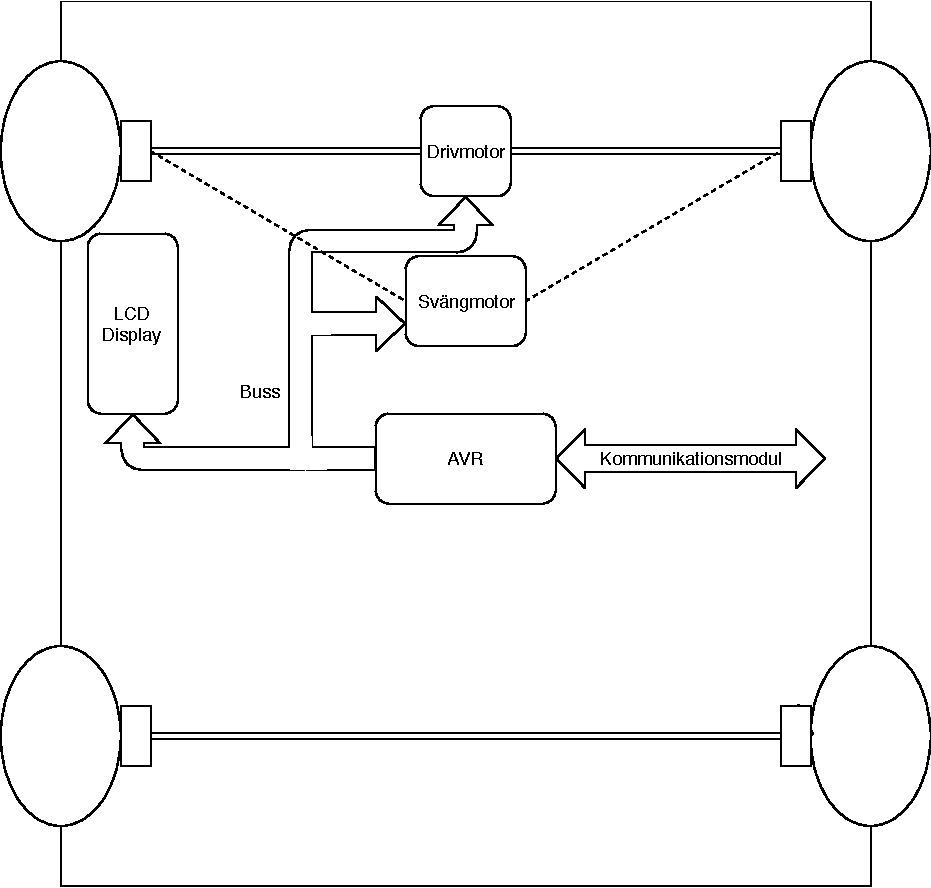
\includegraphics[width=0.6\linewidth]{systemskiss/figures/styrmodul.pdf}
    \caption{Övergripande bild över styrmodulen}
    \label{fig:styrskiss}
\end{figure}

Processorn i modulen har i uppgift att skicka ut rätt styrparameterar till
bilens motorer. Det ska ske via en databuss som inte bara leder till motorerna
utan också en lcd-skärm. På skärmen ska det vara möjligt att visa parametrarna i realtid vilket underlättar felsökning. Figur \ref{fig:styrskiss} är en grov bild på hur modulen ser ut och hur komponenterna är sammankopplade.

\end{document}

